%!TEX root = ../dissertation.tex
\begin{savequote}[75mm]
Knowledge knows no bounds.
%\qauthor{Creator}
\end{savequote}

\chapter{Theory and Motivation}
%\newthought{There's something out there that we don't know.} 

%%%%%%%%%%%%%%%%
%%%%%%%%%%%%%%%%
\section{The Standard Model and the Higgs boson}
\paragraph{}
The Standard Model (SM) ~\cite{Pdg,Griffiths,Tully,Schwartz} is a quantum field theory describing the interactions of elementary particles through the strong, weak, and electromagnetic forces. 
The elementary particles and their properties are shown in Figure~\ref{fig:SM}. 
So far, the SM predictions of particle interactions agree extremely well with almost all experimental observations.

\begin{figure}[htbp!]
  \centering
  \captionsetup{justification=centering}
  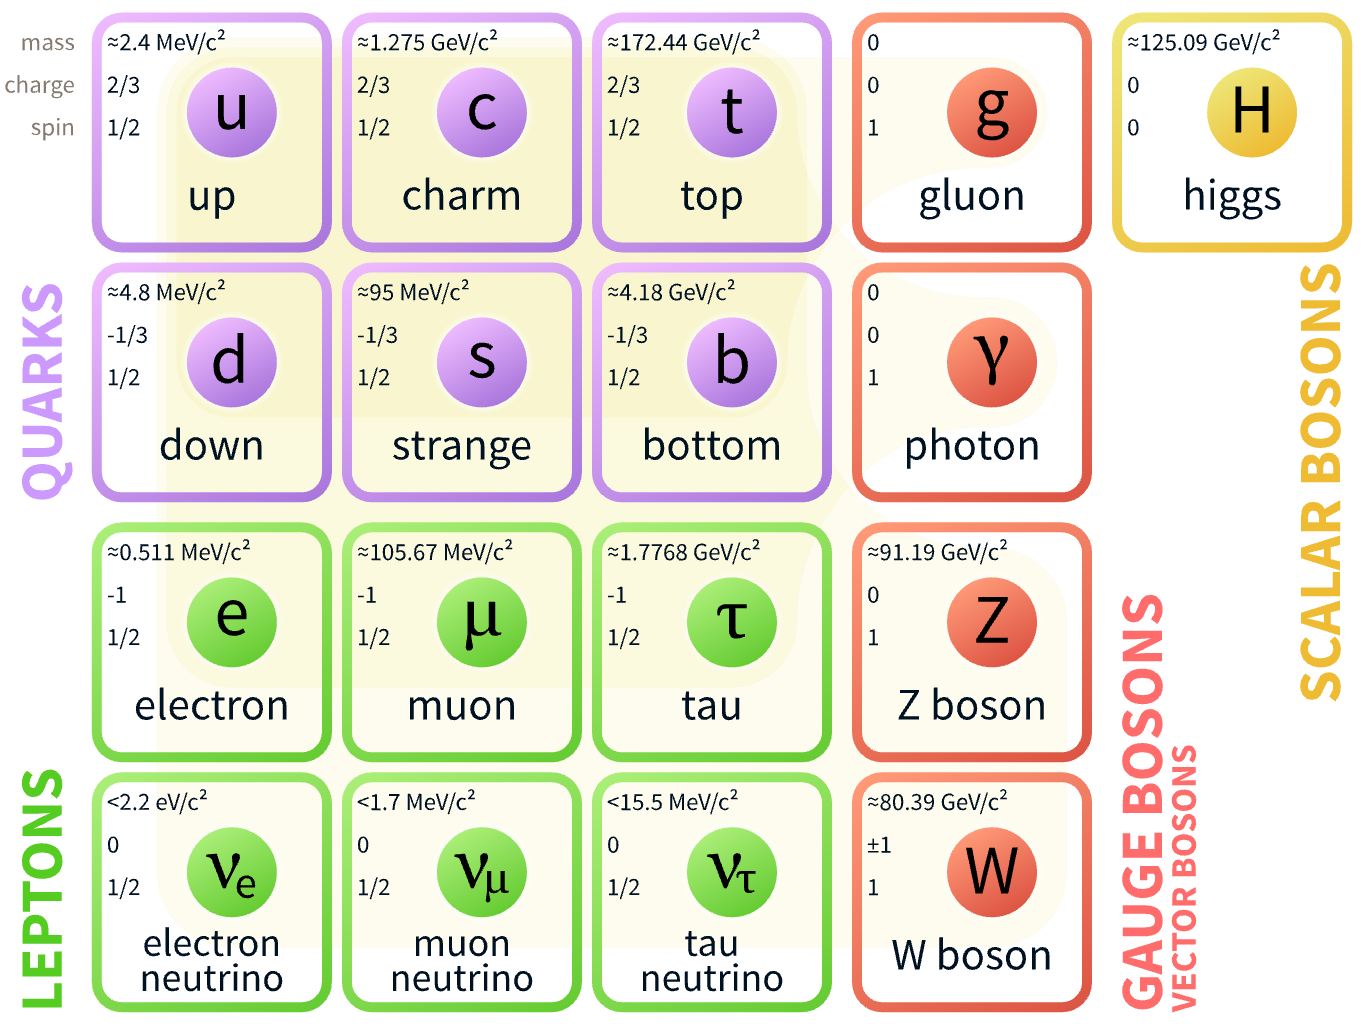
\includegraphics[width=0.6\textwidth]{figures/theory/SM}
  \caption{Fermions and bosons of the Standard Model and their properties~\cite{Pdg}, where all  values are measured experimentally.}
  \label{fig:SM}
\end{figure}

\paragraph{}
%However, in SM, due to the gauge invariance under $SU(2)_{L}$, fermions have to be massless in order to have pure left handed states. 
%The bosons must also be massless as required by the gauge principle. 
In the SM, the Higgs mechanism introduces a complex scalar Higgs field, $\phi$, with nonzero vacuum expectation values. The scalar Higgs potential is $V(\phi) = -\nu^2\lambda_{\rm \nu} \phi^{\dagger}\phi + \lambda_{\rm \nu}(\phi^\dagger\phi)^2$. Through spontaneous symmetry breaking, $W^{\pm}$ and $Z$ bosons acquire their masses.  This process also predicts an extra scalar, the Higgs boson. The SM Lagrangian containing Higgs couplings, $\mathcal{L}_{\rm Higgs}$, is shown in Equation~\ref{eqn:higgspotential}.
\begin{equation}
\label{eqn:higgspotential}
% V(\phi_{h}) = \lambda \nu^2 \phi_{h} ^2  + \lambda \nu \phi_{h} ^3  + \frac{1}{4}\lambda \phi_{h} ^4 
\mathcal{L}_{\rm Higgs} = -\lambda_{hf\bar{f}} hf\bar{f} + \delta_{V} V_{\rm\mu} V^{\rm\mu}\left(\lambda_{\rm hVV} h + \lambda_{\rm hhVV}h^2\right) + \lambda_{\rm hh}h^2 + \lambda_{\rm hhh}h^3 + \lambda_{\rm hhhh}h^4 
\end{equation}
where 
\begin{itemize}
	\item $\rm\nu \sim 246$ \GeV, is the non-zero expectation value of the Higgs field;\
	\item $\lambda_{\rm \nu} \sim -0.13$, the coefficient for the quartic potential term, is constrained from Higgs mass;
  \item $m_{\rm h} = \sqrt{2\lambda_{\rm \nu}}\nu = 125.09 \pm 0.24$ \GeV, is the Higgs mass; this was discovered in 2012\cite{ATLASHiggsDisc, CMSHiggsDisc}; 
	\item $V = W^{\pm}$ or $Z$, $\delta_{W} = 1$, $\delta_{Z} = \frac{1}{2}$;
	\item $\lambda_{hf\bar{f}} = \frac{m_{\rm f}}{\rm\nu}$, is the Higgs to fermion coupling; $m_{\rm f}$ is the mass of the fermion;
	\item $\lambda_{\rm hVV} = \frac{2m_{\rm V}^2}{\rm\nu}$, is the Higgs to boson coupling; $m_{\rm V}$ is the mass of the boson;
	\item $\lambda_{\rm hhVV} = \frac{m_{\rm V}^2}{\rm\nu^2}$, is the Higgs-Higgs to boson-boson coupling;
	\item $\lambda_{\rm hh} = \frac{m_{\rm h}^2}{2}$, is the Higgs mass term;
	\item $\lambda_{\rm hhh} = \frac{m_{\rm h}^2}{2\rm\nu} = \lambda_{\rm \nu} \nu$, or $\lambda_{\rm hhh}$, is the Higgs self-coupling;
	\item $\lambda_{\rm hhhh} = \frac{m_{\rm h}^2}{8\rm\nu^2}$, is the Higgs quartic-coupling.
\end{itemize}
%%%%%%%%TO DO%%%%%%%%
%%%Melissa want pictures of them
%%%%%%%%%%%%%%%%%%%%%%%%
\paragraph{}
$\lambda_{\rm hhh}$ in Equation~\ref{eqn:higgspotential} has not been experimentally measured. 
The SM predicts $\lambda_{\rm hhh} = \frac{m_{\rm h}^2}{2\rm\nu}$, which is referred to as \textbf{$\lambda_{\rm SM}$} in this thesis. 
Measuring $\lambda_{\rm hhh}$ directly probes the quartic term in the Higgs potential.
%A different coupling from $\lambda_{\rm SM}$ is usually referred as just $\lambda$. 
Also, the $\lambda_{\rm hhh}h^3$ term enables a double Higgs production channel within the SM. 
Double Higgs production is also known as \textit{di-Higgs} or \textit{Higgs pair production}.

%Di-Higgs final states will provide complementary information from single Higgs physics at the LHC.
%Measuring this coefficient is one of the major tasks of experimental particle physics program.


%%%%%%%%%%%%%%%%
%%%%%%%%%%%%%%%%
\section{Standard Model di-Higgs production}

% \begin{figure}[htbp!]
%   \centering
%   \captionsetup{justification=centering}
%   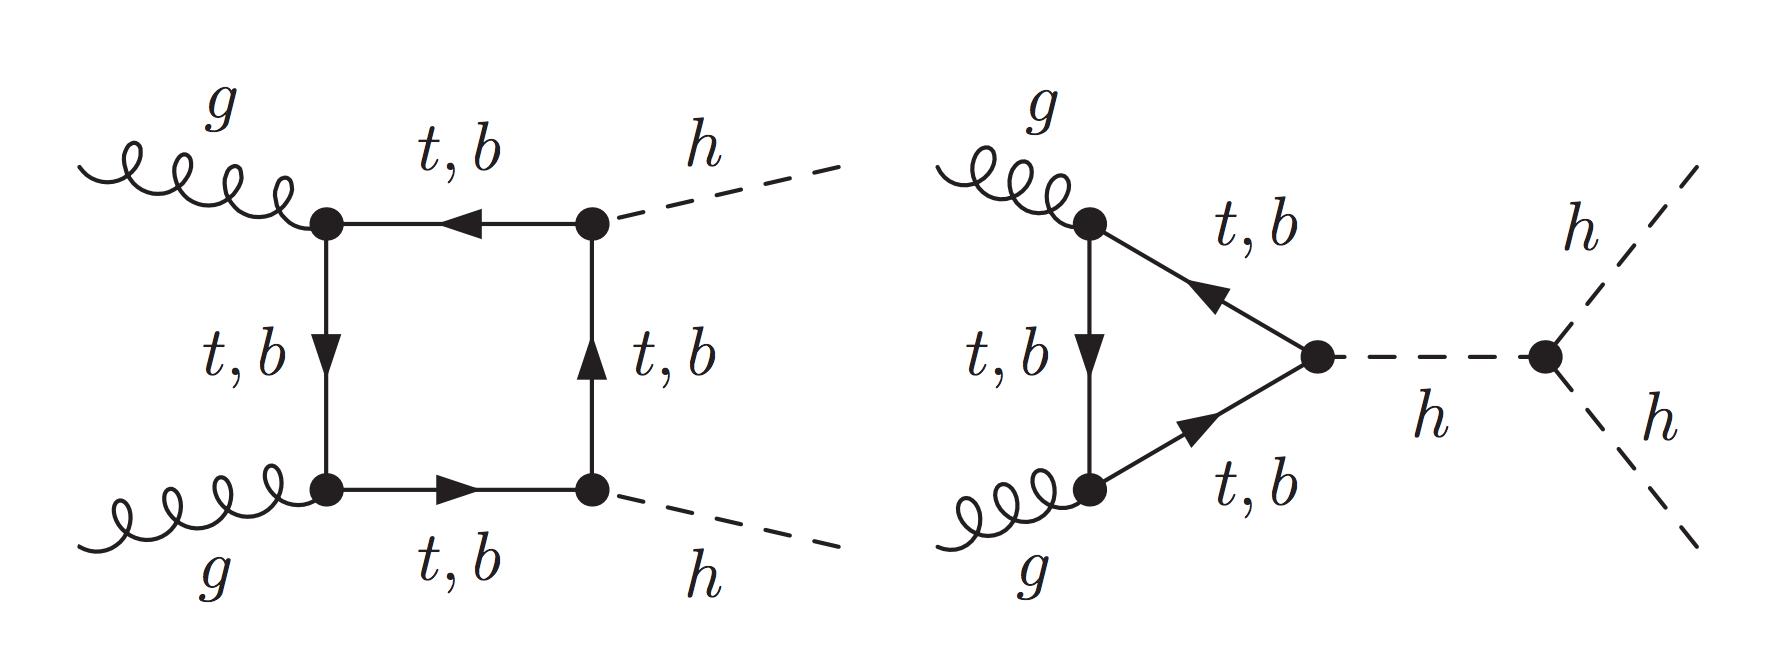
\includegraphics[width=0.7\textwidth]{figures/theory/SM_HH}
%   \caption{Feynman diagrams contributing to di-Higgs production via gluon-gluon fusion, through a $t$ or $b$ quark loop, at leading order. Only the right hand plot probes $\lambda_{hhh}$.}
%   \label{fig:SM_HH}
% \end{figure}

% \paragraph{}
% In the SM, the Higgs boson pair production through the $\lambda_{\rm hhh}$ has an on-shell component and a large off-shell component. The on-shell is strongly disfavored, requiring two off-shell Higgs bosons in the final state. The sensitivity region to the trilinear coupling production as in ~\ref{fig:SM_HH_tri}, is mainly in the kinematic region where the two Higgs boson in the final state are on-shell and the Higgs boson acts as a propagator (off-shell).

\paragraph{}
There are two main di-Higgs production diagrams at the LHC, both shown in Figure~\ref{fig:SM_HH}. In the gluon-gluon  fusion process, di-Higgs are produced through a box or a triangle loop. 
Only the triangle loop Figure~\ref{fig:SM_HH_tri} probes the $\lambda_{hhh}$. 
In the triangle diagram, the middle Higgs boson acts as a propagator (off-shell), and the two Higgs bosons in the final state are on-shell. 
The diagram with an on-shell middle Higgs and two off-shell Higgs bosons in the final state is strongly suppressed~\cite{Pdg}.
The box and triangle diagrams interfere destructively, which makes the overall production rate smaller than what would be expected in the absence of a $\lambda_{hhh}$ term.

\begin{figure}[htbp!]
\centering
\captionsetup{justification=centering}
    \begin{subfigure}[b]{0.4\textwidth}
        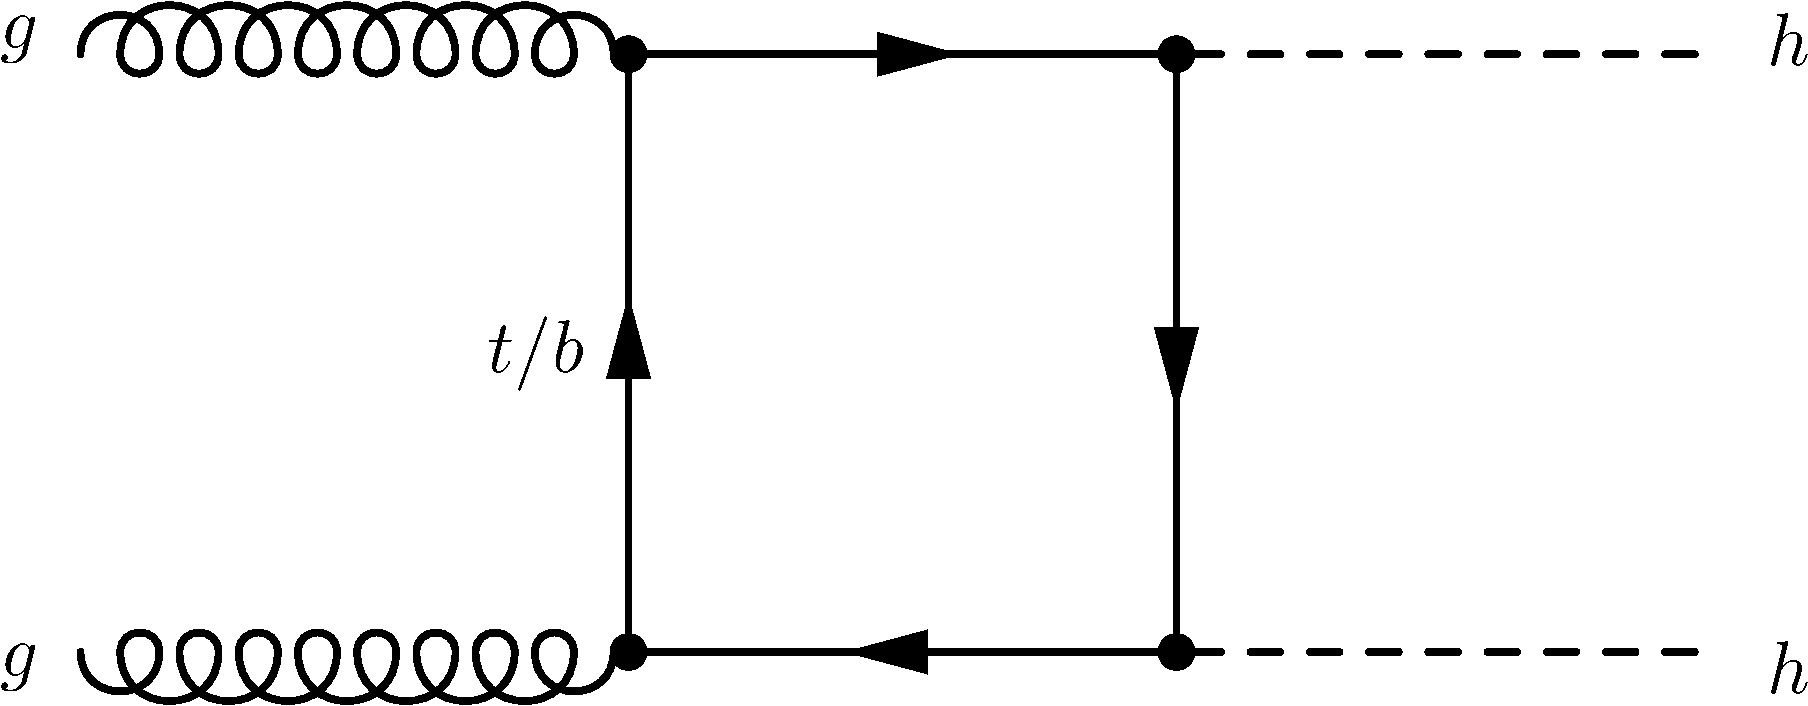
\includegraphics[width=\textwidth]{figures/theory/SM_HH_box}
        \caption{Box diagram}
        \label{fig:SM_HH_box}
    \end{subfigure}
    \quad
    \begin{subfigure}[b]{0.4\textwidth}
        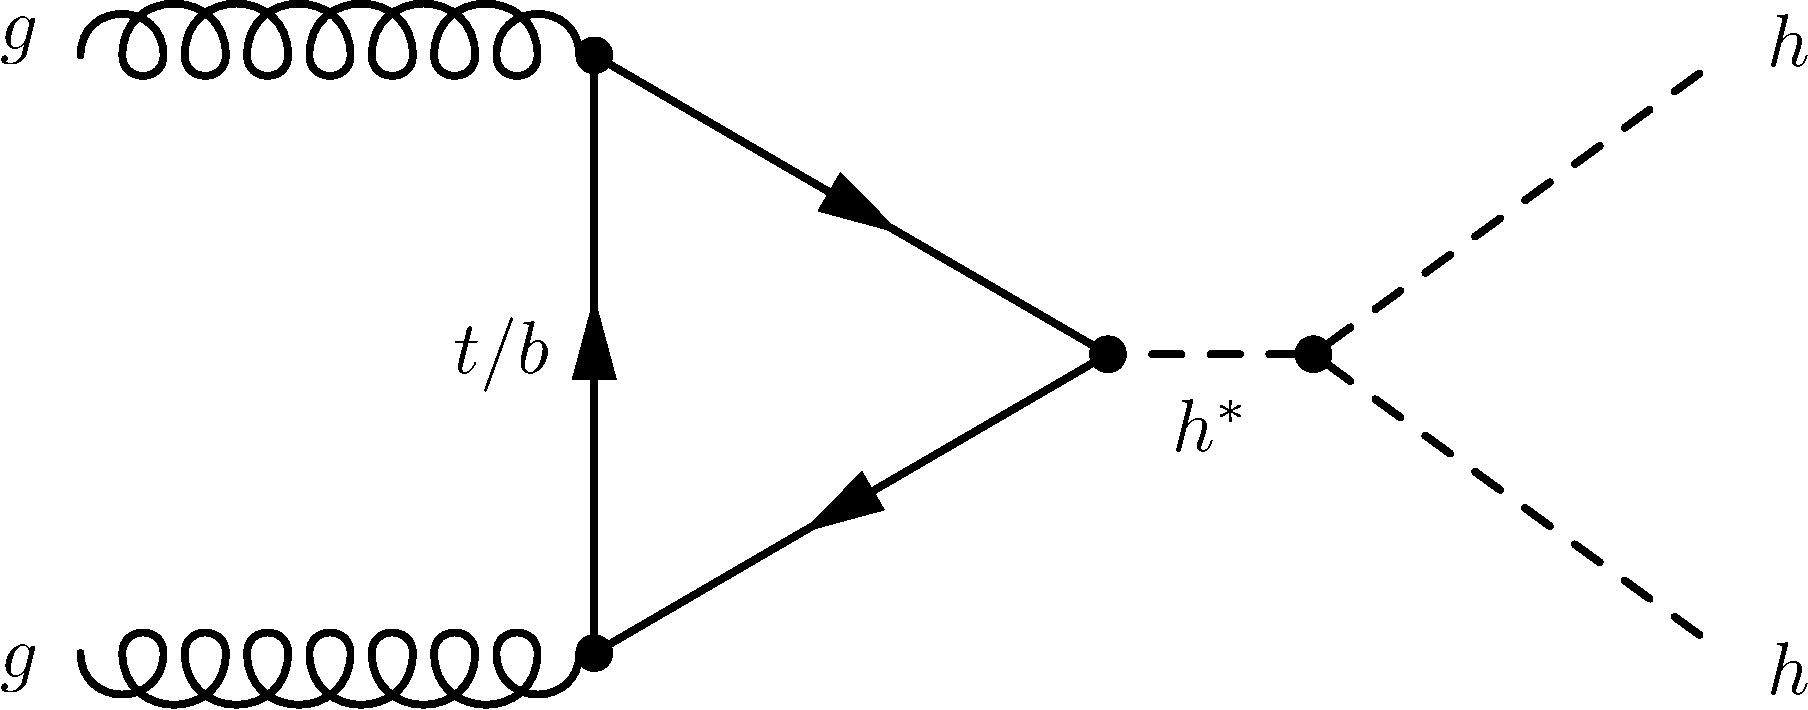
\includegraphics[width=\textwidth]{figures/theory/SM_HH_tri}
        \caption{Triangle diagram}
        \label{fig:SM_HH_tri}
    \end{subfigure}
\caption{Leading order Feynman diagrams contributing to di-Higgs production via gluon-gluon fusion, through the Higgs-fermion Yukawa interactions in Figure~\ref{fig:SM_HH_box} and the Higgs boson self-coupling in Figure~\ref{fig:SM_HH_tri}. Only Figure~\ref{fig:SM_HH_tri} probes $\lambda_{hhh}$.}
\label{fig:SM_HH}
\end{figure}

\paragraph{}
Many other different production modes of di-Higgs exist. 
The Feynman diagrams for VBF production are shown in Figure~\ref{fig:SM_HH_VBF}. 
Figure~\ref{fig:SM_HH_xsec}~\cite{Frederix:2014hta} compares the cross sections of gluon-gluon fusion, vector boson fusion (VBF), top-pair, $W^{\pm}$, $Z$ and single-top associated di-Higgs production.
It shows that gluon-gluon fusion is the dominant production channel for di-Higgs at $pp$ colliders. 

\begin{figure}[htbp!]
  \centering
  \captionsetup{justification=centering}
  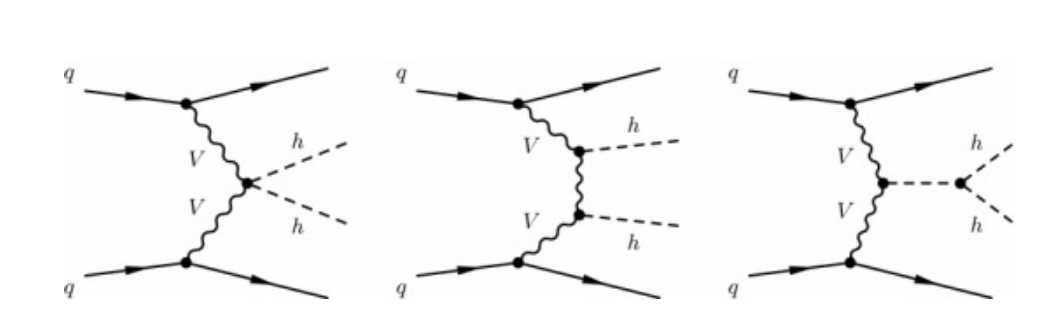
\includegraphics[width=0.7\textwidth]{figures/theory/SM_HH_VBF}
  \caption{Leading order Feynman diagrams contributing to Higgs pair production via VBF.}
  \label{fig:SM_HH_VBF}
\end{figure}

\begin{figure}[htbp!]
  \centering
  \captionsetup{justification=centering}
  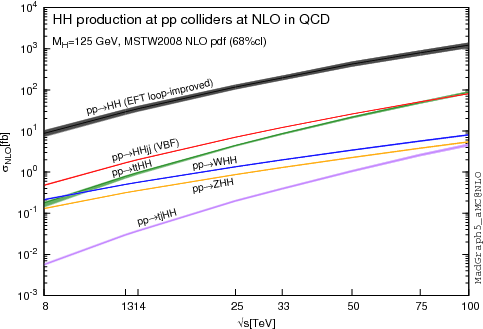
\includegraphics[width=0.7\textwidth]{figures/theory/HH_xsec}
  \caption{Total cross sections (y-axis) at the NLO in QCD for the six largest di-Higgs production channels at $pp$ colliders for different energy (x-axis). Gluon-gluon fusion, VBF, top-pair, $W^{\pm}$, $Z$ and single-top associated di-Higgs productions are shown. The thickness of the lines corresponds to the uncertainties added linearly. $H$ refers to the SM Higgs.}
  \label{fig:SM_HH_xsec}
\end{figure}

\paragraph{}
\label{par:diHiggs-crosssection}
For $pp$ collisions at $\sqrt{s}=13$ \TeV, the total cross section for SM di-Higgs production~\cite{LHCYellow} is evaluated at next-to-next-to-leading order (NNLO) with the summation of logarithms at next-to-next-leading-logarithm (NNLL) accuracy and including finite top-quark mass effects at next-to-leading order (NLO).
There are uncertainties from energy scale and parton distributions functions (PDF). 
The production cross section, broken down by different production modes, are as follows:
\begin{itemize}
  \item Gluon gluon fusion: $\sigma_{gg \to HH} = 33.49^{+ 4.3 \%}_{-6.0 \%} \pm 2.1\%$ fb. %\pm 2.3\%$ $\alpha_s$
  \item Vector boson fusion: $\sigma_{VBF \to HH} = 1.62^{+ 2.3 \%}_{-2.7 \%} \pm 2.3\%$ fb.
  \item Gluon gluon fusion to Triple-Higgs: $\sigma_{gg \to HHH} = 0.06332 ^{+ 16.1 \%}_{-14.1 \%} \pm 3.4\% $ fb.
\end{itemize}
A femtobarn (fb) is a unit of area equal to $10^{-43}$ m$^2$.
This means with the full 2015 and 2016 36 \ifb dataset, the SM expectation is around one thousand di-Higgs events and only two triple Higgs events.



%%%%%%%%%%%%%%%%
%%%%%%%%%%%%%%%%
\section{Beyond the Standard Model di-Higgs production}
\paragraph{}
The SM has had many successful experimental predictions, yet the Higgs boson mass at $125$ \GeV~ requires extreme fine-tuning for radiative corrections~\cite{Pdg}. 
The presence of new physics at the \TeV~ scale would help solve this unnatural fine-tuning problem.

\paragraph{}
Beyond the Standard Model (BSM) physics could significantly enhance both resonant and non-resonant production of di-Higgs at the LHC.
Non-resonant production generally refers to modifications of the Higgs couplings, either the Higgs self-coupling or the Higgs-top couplings. 
Resonant production refers to the case when a particle with invariant mass greater than twice the Higgs mass decays directly into two Higgs bosons. 
Non-resonant and resonant production also translate to different di-Higgs invariant mass distributions at truth level.
In the non-resonant case, the invariant mass distribution has no clear peak, whereas in the resonant case, the invariant mass distribution usually forms a peak with a model dependent width. 

\begin{figure}[htbp!]
\centering
\captionsetup{justification=centering}
    \begin{subfigure}[b]{0.3\textwidth}
        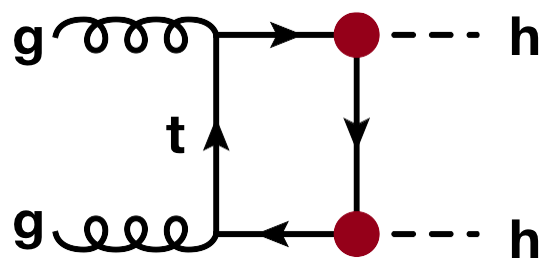
\includegraphics[width=\textwidth]{figures/theory/BSM_HH_box}
        \caption{$H$-fermion vertices variations}
        \label{fig:BSM_HH_box}
    \end{subfigure}
    \quad
    \begin{subfigure}[b]{0.3\textwidth}
        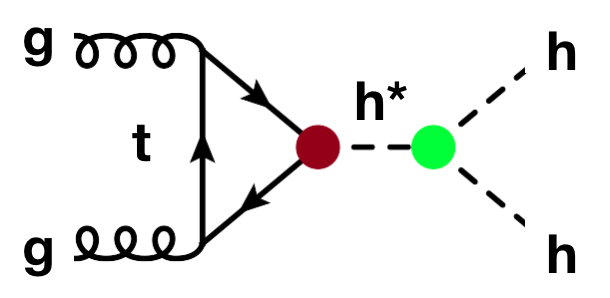
\includegraphics[width=\textwidth]{figures/theory/BSM_HH_tri}
        \caption{Higgs self-coupling variations}
        \label{fig:BSM_HH_tri}
    \end{subfigure}
    \quad
    \begin{subfigure}[b]{0.3\textwidth}
        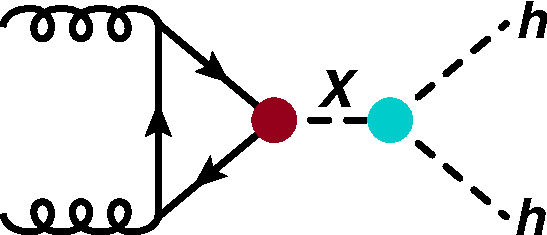
\includegraphics[width=\textwidth]{figures/theory/BSM_HH_X}
        \caption{An intermediate resonance, X}
        \label{fig:BSM_HH_X}
    \end{subfigure}
\caption{BSM Higgs boson pair production: non-resonant production proceeds through changes in the SM Higgs couplings in Figure~\ref{fig:BSM_HH_box} and Figure~\ref{fig:BSM_HH_tri}, resonant production proceeds through Figure~\ref{fig:BSM_HH_X} an intermediate resonance, X. $H$ and $h$ both refers to the SM Higgs.}
\label{fig:BSM_HH}
\end{figure}


%%%%%%%%%%%%%%%%
%%%%%%%%%%%%%%%%
\subsection{BSM non-resonant di-Higgs}
\paragraph{}
Enhanced non-resonant Higgs boson pair production is predicted in many models. 
BSM models featuring direct $t\bar{t}\hh$ vertices \cite{Grober:2010yv, Contino:2012xk} or new light colored scalars \cite{PhysRevD.86.095023} could augment the vertex strength, shown as red circles in Figure~\ref{fig:BSM_HH}. 
A direct modification of the Higgs self-coupling coefficient in Eq~\ref{eqn:higgspotential}, from $\lambda_{\rm sm}hhh$ to $\lambda hhh$, is also possible. 
This is shown as a green circle in Figure~\ref{fig:BSM_HH_tri}. 

\begin{figure}[htbp!]
  \centering
  \captionsetup{justification=centering}
  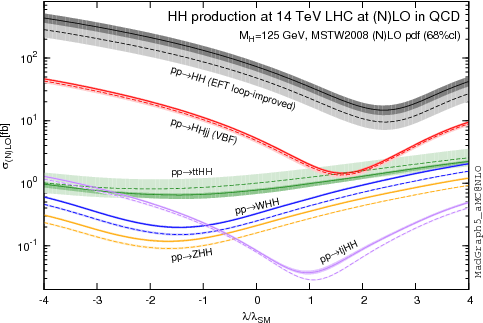
\includegraphics[width=0.7\textwidth]{figures/theory/HH_lam}
  \caption{Total cross sections (y-axis) at the LO and NLO in QCD for di-Higgs production channels, at the LHC $\sqrt{s} = 14$ \TeV~ as a function of the self-interaction coupling $\lambda$ (x-axis) . The dashed (solid) lines and light- (dark-) color bands correspond to the LO (NLO) results and to the scale and PDF uncertainties added linearly. The SM values of the cross sections are obtained at $\frac{\rm \lambda}{\rm \lambda_{\rm SM}} = 1$, indicated by the red vertical line. $H$ refers to the SM Higgs.}
  \label{fig:SM_HH_lam}
\end{figure}

\paragraph{}
The non-resonant di-Higgs enhancement is usually described by the di-Higgs cross section ratio between a BSM $\lambda$ coupling scenario and the $\lambda_{\rm SM}$ coupling scenario.
$\frac{\rm \lambda}{\rm \lambda_{\rm SM}}$ indicates the ratio between the BSM model $\lambda$ and $\lambda_{\rm SM}$.
From SM electroweak measurements, the self coupling term is constrained to $-14 \leq \frac{\rm \lambda}{\rm \lambda_{\rm SM}} \leq 17.4$~\cite{Kribs:2017znd}. 
Variations of $\lambda$ have a non-trivial effect on di-Higgs production cross section, shown in Figure~\ref{fig:SM_HH_lam}~\cite{Frederix:2014hta}. 
In the regime of relatively high trilinear coupling, $10 < |\frac{\rm \lambda}{\rm \lambda_{\rm SM}}|$, the interference between the two diagrams is dominated by the trilinear coupling term. 
A simple limit on $\frac{\rm \lambda}{\rm \lambda_{\rm SM}}$ can be set based on the observed cross section limit.



%%%%%%%%%%%%%%%%
%%%%%%%%%%%%%%%%
\subsection{BSM resonant di-Higgs}
\paragraph{}
%In summary, resonant di-Higgs searches could test many models including extra dimensions and Supersymmetry.
Theoretically, it is relatively easy to introduce new heavy resonances that interact with the SM through the Higgs as a mediator.
This usually results in resonant di-Higgs production. 
With the increase in center of mass collision energy from $8$ \TeV~ to $13$ \TeV~ in Run 2 of the LHC, the production cross section for particles with \TeV~ mass grows dramatically, as shown in Figure~\ref{fig:lumi_ratio}.
In the case of a $2$\TeV $M_X$, the cross section gain is almost a factor of $10$. 
Therefore, it is particularly important to focus on resonant searches in the region above $1$ \TeV.

\begin{figure}[htbp!]
  \centering
  \captionsetup{justification=centering}
  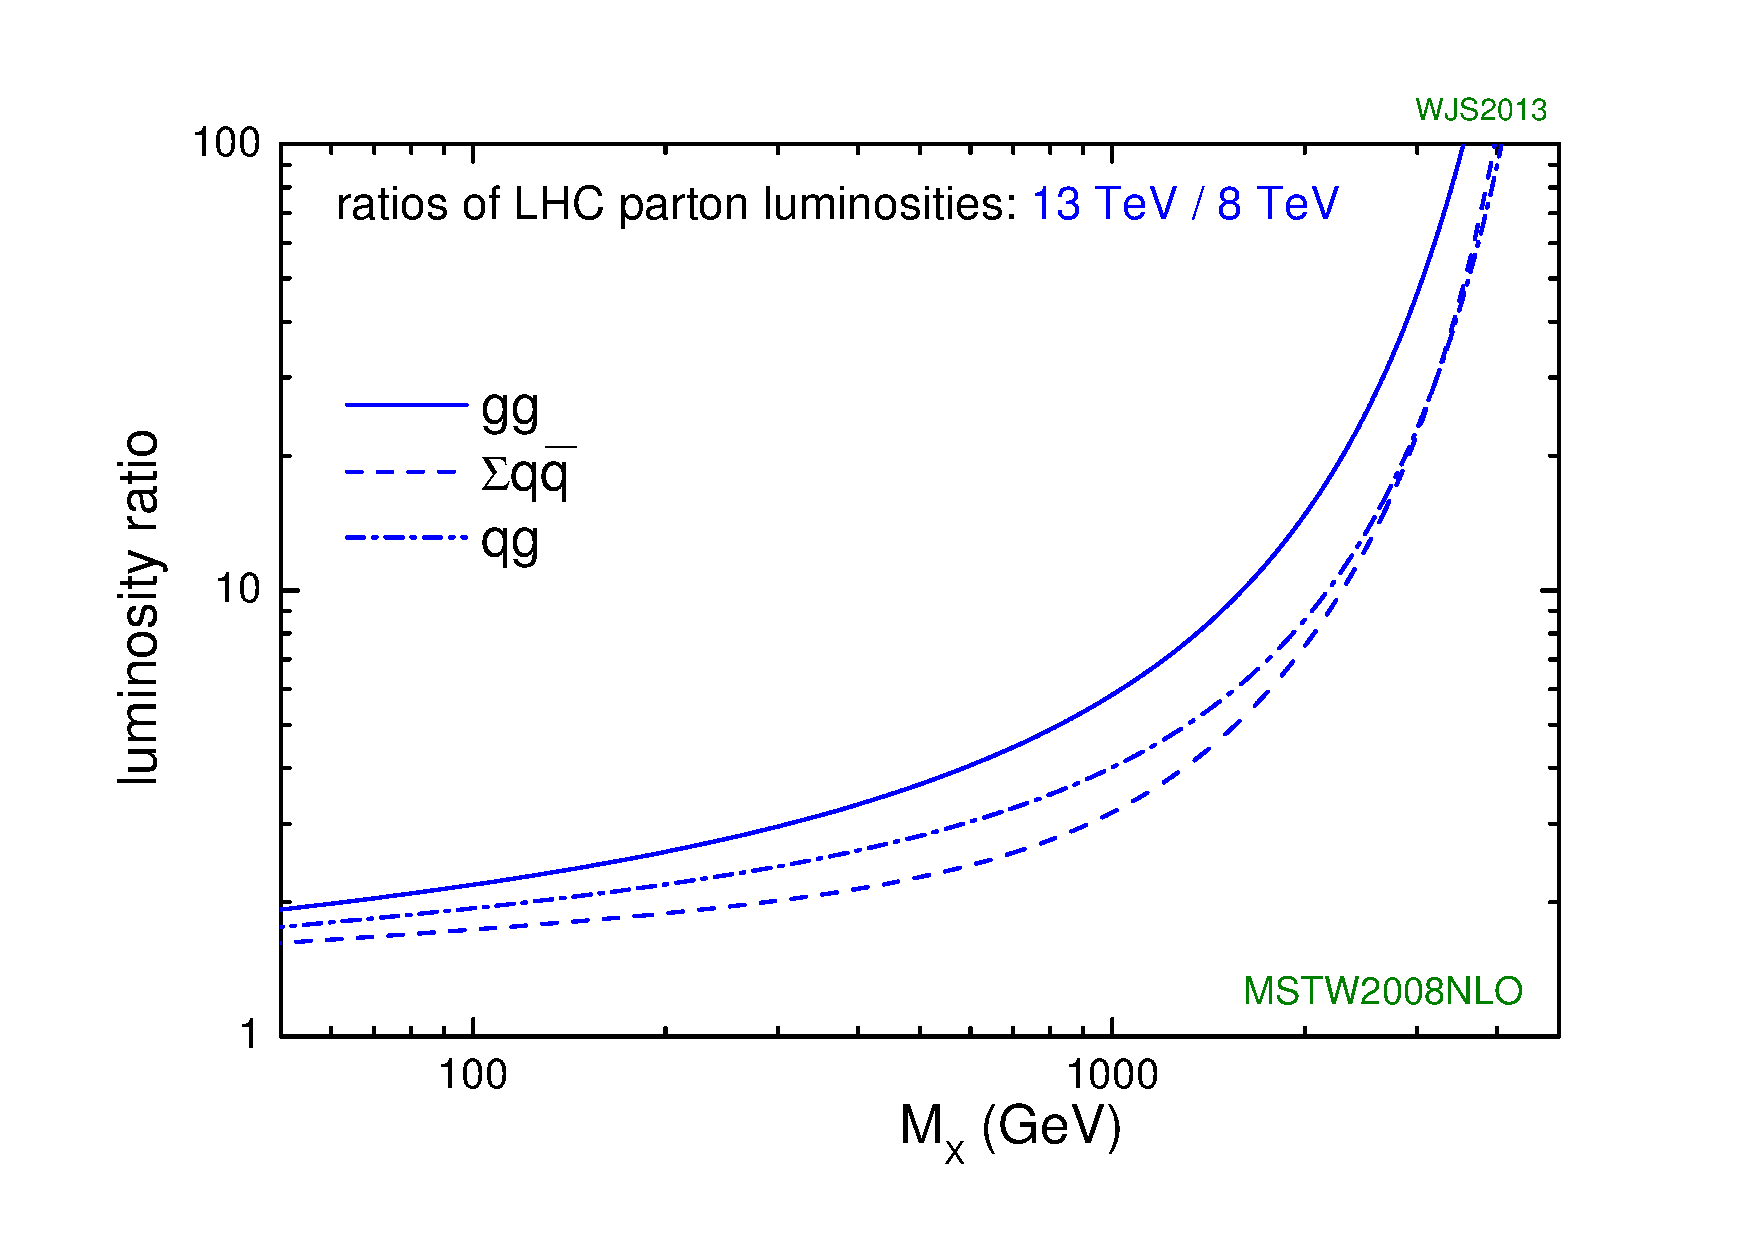
\includegraphics[width=0.6\textwidth]{figures/theory/lhclumi7813_2013_v1}
  \caption{Parton luminosity ratios as a function of resonance mass, $M_{X}$, for $13/8$ \TeV~\cite{LumiRatio}. $1$, $2$, and $3$ ~\TeV $M_{X}$ ratios are indicated by red lines. For a $2$ \TeV $X$, the luminosity ratio is almost 10.}
  \label{fig:lumi_ratio}
\end{figure}

\paragraph{}
Resonant Higgs boson pair production is also predicted by many models. Extensions of the Higgs sector, such as two-Higgs-doublet models (2HDM)~\cite{PhysRevD.8.1226, Branco:2011iw}, propose the existence of a heavy spin-0 scalar $H$ that can decay into two Higgs bosons. 
The bulk Randall-Sundrum model~\cite{Agashe:2007zd, Fitzpatrick}, which features spin-2 Kaluza-Klein gravitons, \Grav, could also subsequently decay to pairs of Higgs bosons. 
These proposed heavy particles, heavy CP-even scalar $H$ and \Grav, are represented as X in Figure~\ref{fig:BSM_HH_X}.
In model dependent searches, based on fixed assumptions of the resonant particles' branching ratio, other searches for resonances decaying into $VV$ or \ttbar~ are more sensitive compared to di-Higgs searches~\cite{Cavaliere:2203605}. 
In order to fully constrain the BSM physics production and decay phase space, di-Higgs search results are interpreted in different models, covering both narrow and wide resonances.

\paragraph{}
The Randall-Sundrum model proposes a five-dimensional warped space-time that contains two manifolds: one where the force of gravity is very strong and a second manifold at the \TeV~ scale corresponding to the known SM sector.
The experimental consequence of this theory is a series of widely mass-spaced Kaluza-Klein graviton resonances, \Grav. 
In cases where the fermions are localized to the SM manifold, production of gravitons from fermion pairs is suppressed and the primary mode of production of \Grav is gluon-gluon fusion. 
These gravitons further decay to two Higgs bosons, with branching fraction ranging from $6.43$\% for gravitons with a mass of $500$ \GeV~ to $7.66\%$ at $3$ \TeV.
Randall-Sundrum models have two free parameters --- the mass of the graviton and $c = k/\bar{M}_{\rm pl}$, where $\bar{M}_{\rm pl}$ is the reduced Planck mass and $k$ is the curvature scale of the extra dimension. 
The width of the graviton increases with both mass and $c$.
In Run 1, the \Grav~ with $c=1.0$ is excluded by searches in di-boson and di-Higgs channels up to $760$ \GeV, as shown in Figure~\ref{fig:run1-RSG}.
Therefore, probing the \TeV~ region is promising in the LHC Run 2.

\begin{figure}[htb!]
  \centering
  \hspace{-2cm}
  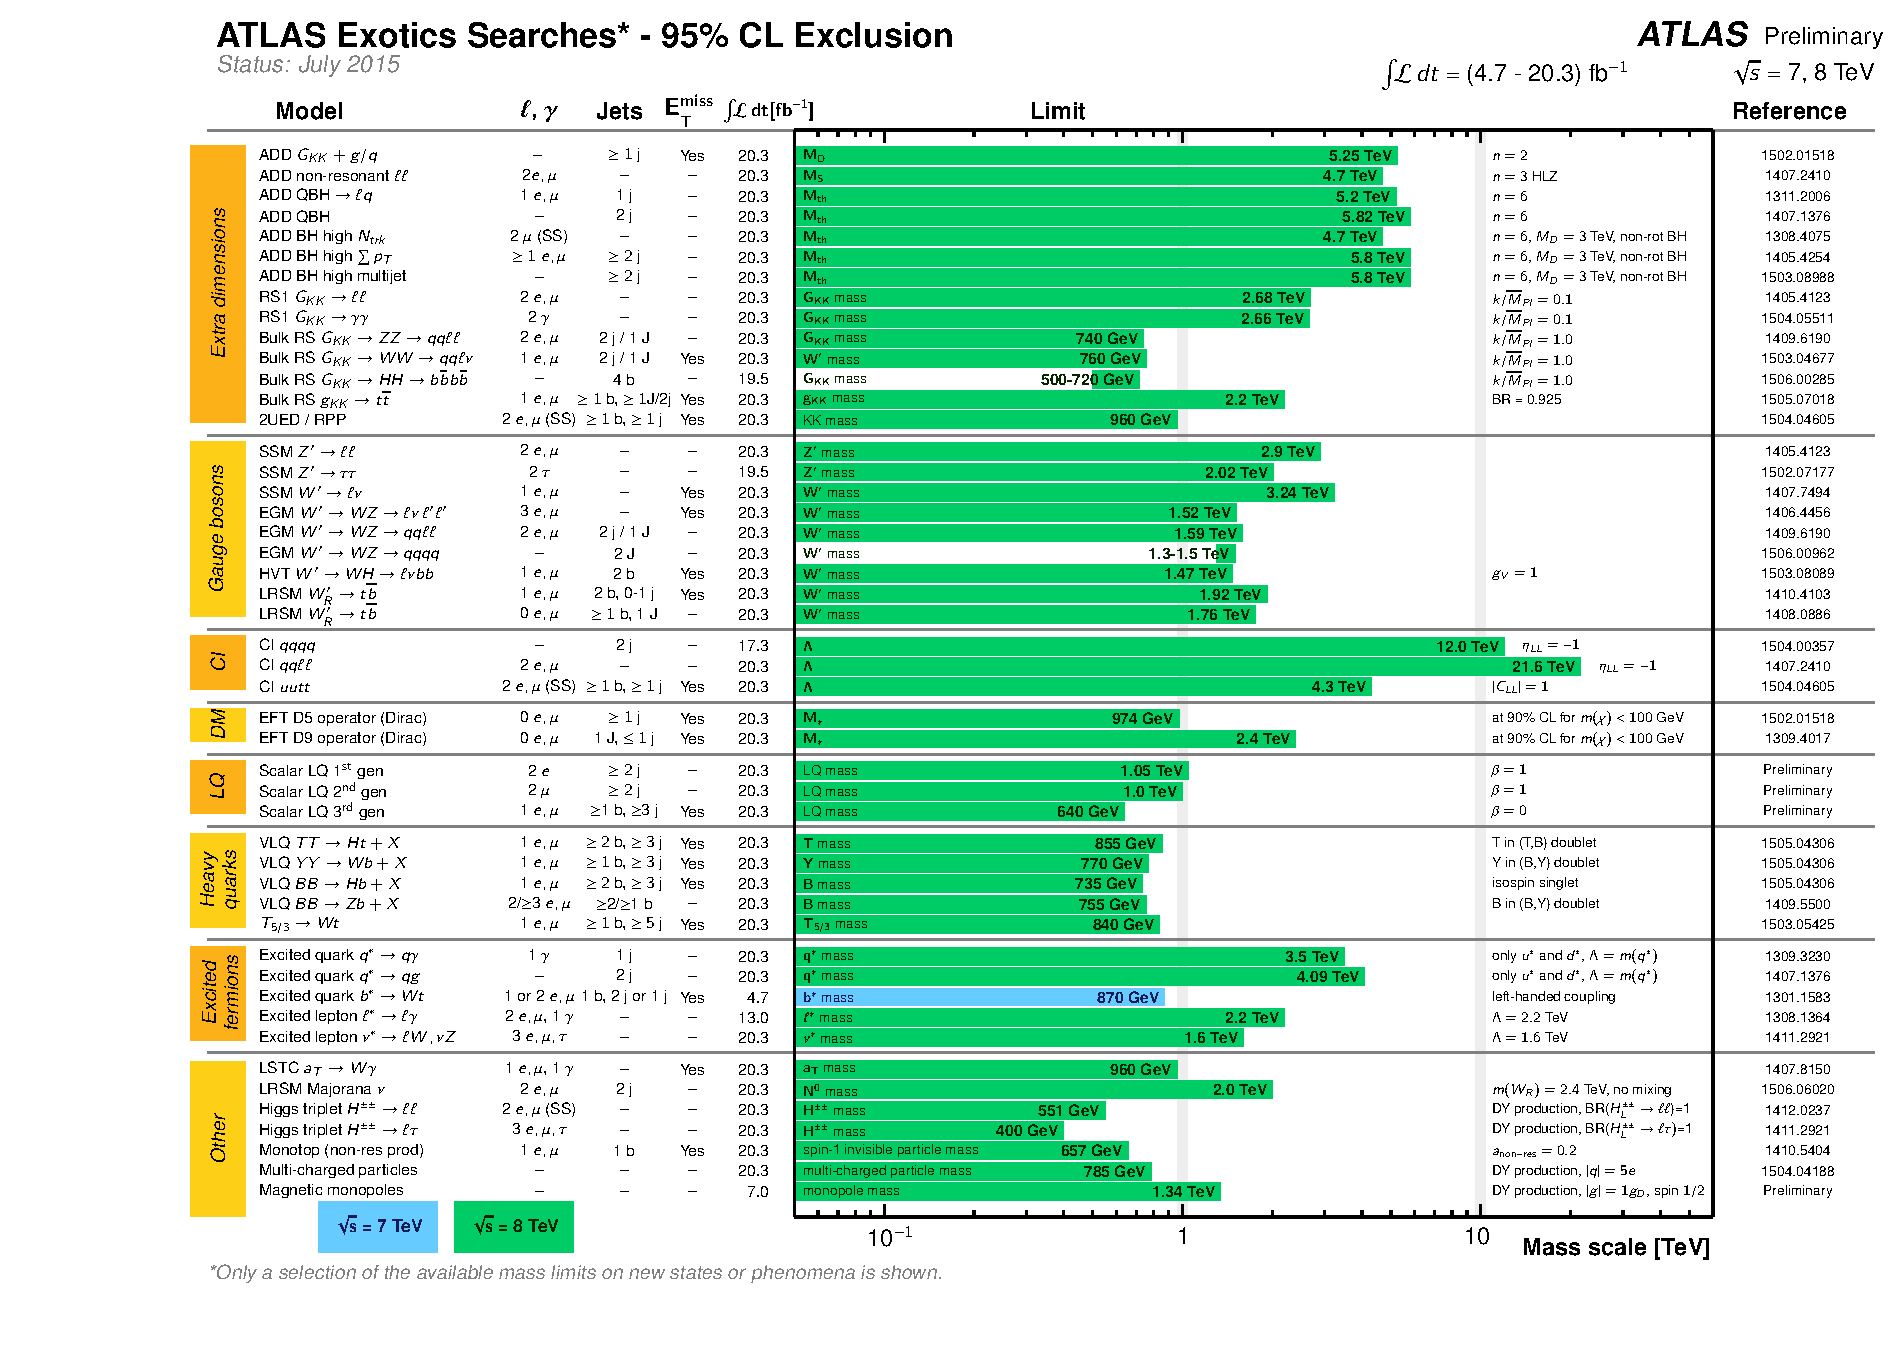
\includegraphics[width=\textwidth]{figures/theory/ATLAS_Exotics_Summary_201507}
  \caption{Reach of ATLAS searches for new phenomena. Only a representative selection of the available results is shown. Blue (green) bands indicate $7$ \TeV~ ($8$ \TeV) data results.}
  \label{fig:run1-RSG}
\end{figure}
%https://atlas.web.cern.ch/Atlas/GROUPS/PHYSICS/CombinedSummaryPlots/EXOTICS/ATLAS_Exotics_Summary/history.html
%https://atlas.web.cern.ch/Atlas/GROUPS/PHYSICS/CombinedSummaryPlots/EXOTICS/ATLAS_Exotics_Summary/ATLAS_Exotics_Summary_201507.pdf

\begin{figure}[htb!]
  \centering
  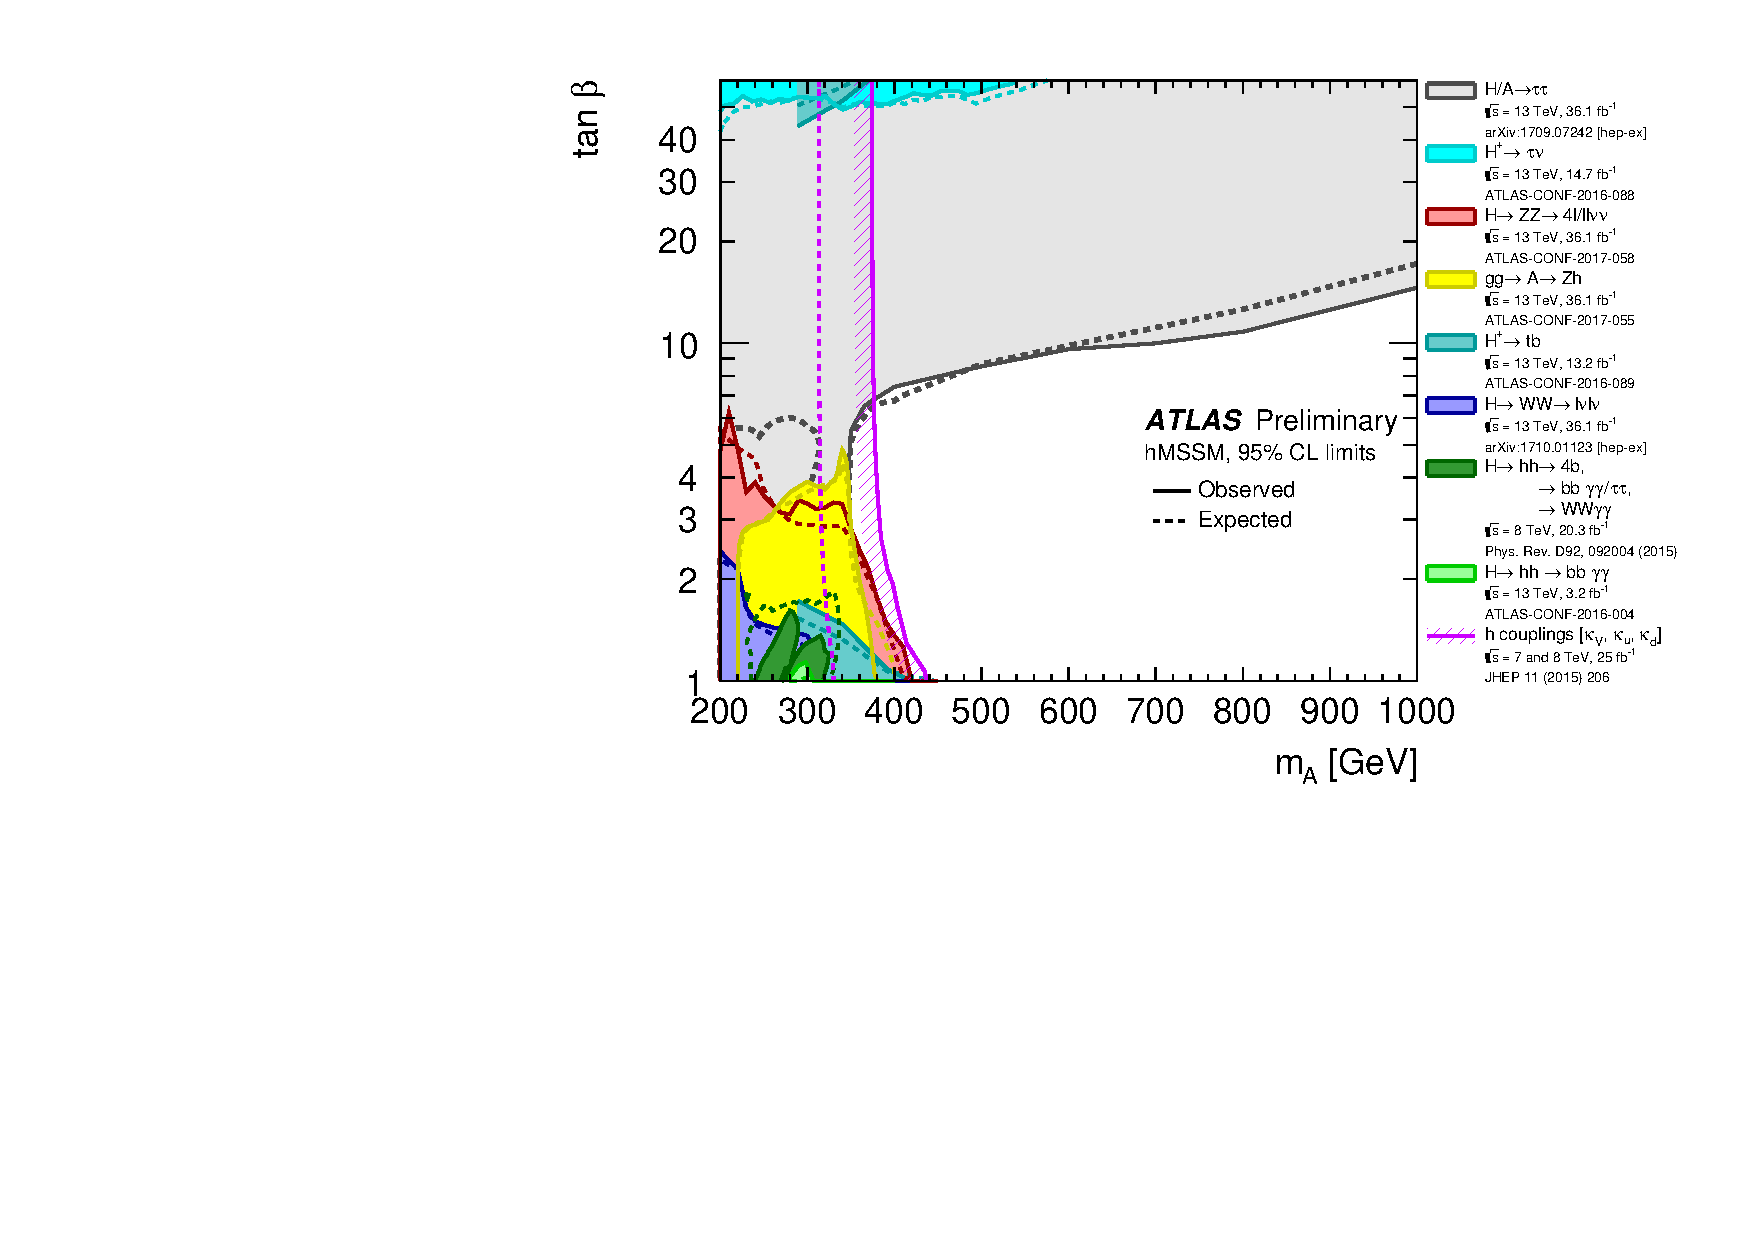
\includegraphics[width=0.6\textwidth, angle=-90]{figures/theory/ATLAS_HIGGS5101_BSM_hMSSM_tanb_vs_mA_Summary_LargeRange}
  \caption{Regions of the [$m_A$, $tan\beta$] plane excluded in the hMSSM model via direct searches for heavy Higgs bosons and fits to the measured rates of observed Higgs boson production and decays. Limits are quoted at $95\%$ CL and are indicated for the data (solid lines) and the expectation for the SM Higgs sector (dashed lines). The light shaded or hashed regions indicate the observed exclusions.}
  \label{fig:run1-2HDM}
\end{figure}

\paragraph{}
The 2HDM is a a simple extension of the SM which has large resonance effects~\cite{LHCYellow}. 
The 2HDM consists of 5 physical Higgs bosons: $h$ (light scalar Higgs), $H$ (heavy scalar Higgs), $A$ (heavy pesudoscalar Higgs), and $H^{\pm}$ (two charged Higgs). 
The 2HDM can introduce tree level flavor changing neutral currents. 
To avoid this obvious contradiction with the SM, models impose discrete symmetries in which the charged fermions only couple to one of the Higgs doublets.
One class of such models is type II 2HDM, in which all positively charged quarks couple to one doublet and the negatively charged quarks and leptons couple to the other. 
The type II model is consistent with the Minimal Supersymmetric Standard Model (MSSM).
Resonant di-Higgs production in 2HDM models can proceed through decays of the heavy CP-even Higgs $H\to hh$. 
The branching ratio for $H\to hh$ depends on the model type as well as the values of $\tan{\beta}$ and $\cos(\beta - \alpha)$. 
$\tan{\beta} = \frac{\rm \nu_{\rm doublet2}}{\rm \nu_{SM}}$ is the ratio of the vacuum expectation values of the two Higgs doublets. 
$\alpha$ is the mixing angle between the heavy $H$ and light $h$ fields. 
The limit where $\cos(\beta - \alpha) = 0$ is called the alignment limit, where the light Higgs $h$ has the same couplings as a SM Higgs.
For a fixed range of $\tan{\beta}$, the phase space close to the alignment limit is unexplored, as shown in Figure~\ref{fig:run1-2HDM}.
Di-Higgs searches have only excluded the low $m_A$ mass regions in Run 1.
It is of particular interest in BSM searches at the LHC Run 2.


%%%%%%%%%%%%%%%%
%%%%%%%%%%%%%%%%
\section{Di-Higgs decay and LHC previous search results}
\label{sec:hhdecay}
\paragraph{}
The Higgs boson has a short lifetime of $1.56 \times 10^{-22}$s.
It decays into other elementary particles as soon as it is produced in $pp$ collisions. 
Therefore, searching for di-Higgs productions requires reconstructing the Higgs boson from its decay products.
Di-Higgs decay modes is a combination of two single Higgs boson decay modes. 
%which is determined by the Higgs coupling terms to fermions and bosons are shown in Equation~\ref{eqn:higgspotential}. 
The branching ratios of different di-Higgs final states are shown in Figure~\ref{fig:HH_BR}.

\begin{figure}[htbp!]
  \centering
  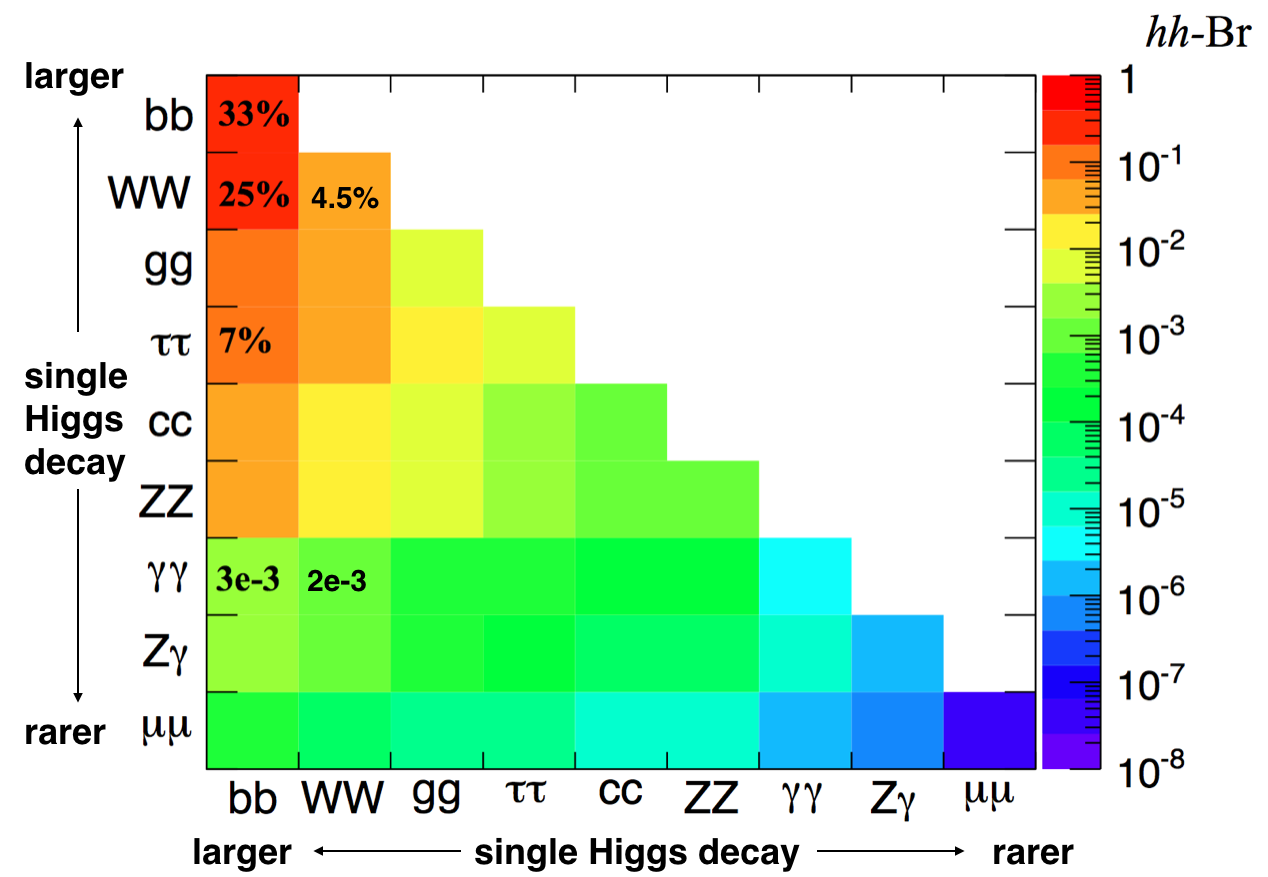
\includegraphics[width=0.6\textwidth]{figures/theory/HH_BR}
  \caption{Summary of di-Higgs final states and their ratios. Top left, \bbbb, has the largest branching ratio.}
  \label{fig:HH_BR}
\end{figure}

\begin{figure}[htbp!]
  \centering
  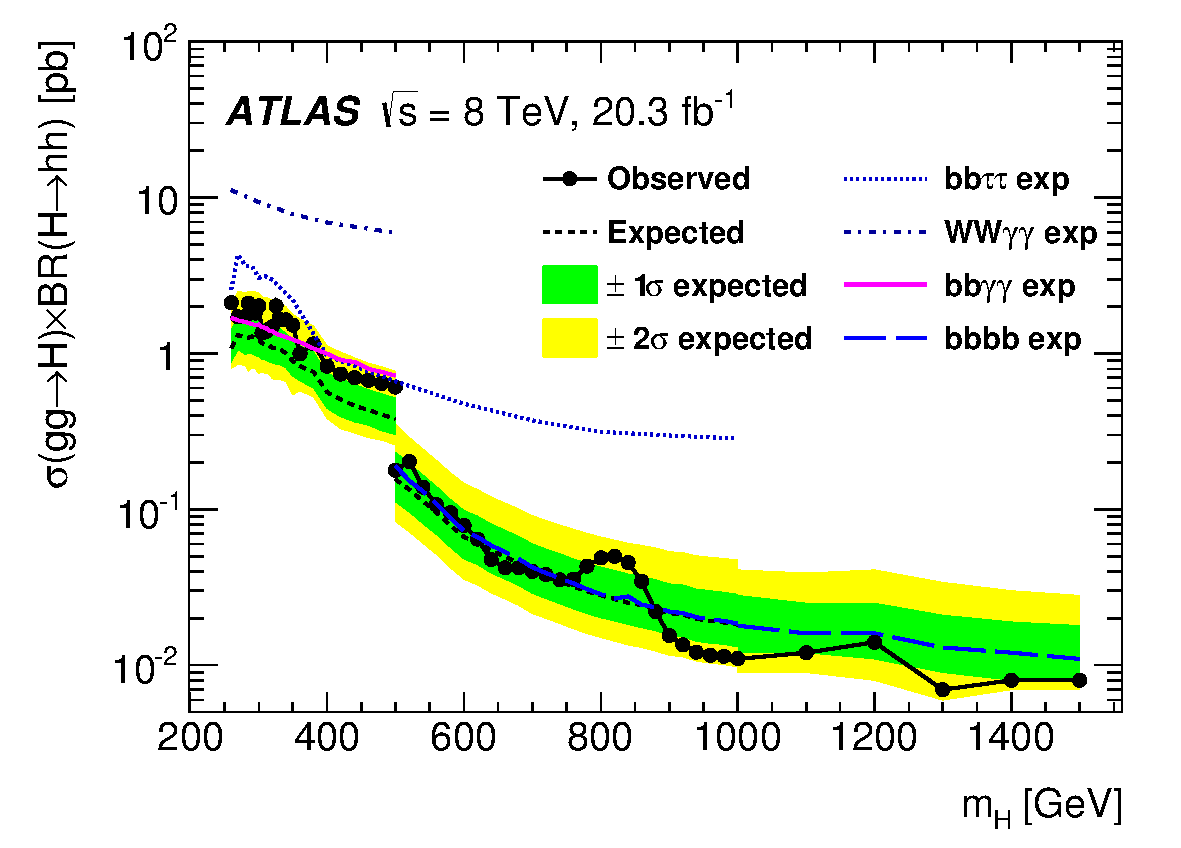
\includegraphics[width=0.6\textwidth]{figures/theory/Run1_ATLAS}
  \caption{The observed and expected $95\%$ CL upper limits of $\sigma(gg \to H) \times BR(H \to hh)$ at $\sqrt{s}=8$\TeV~ as functions of the heavy Higgs boson mass, $m_{H}$, combining resonant searches in Higgs boson pair to \bbtautau~, \WWgg~, \bbgg~, and \bbbb~ final states. The expected limits from individual searches are also shown. The green and yellow bands represent $\pm 1\sigma$ and $\pm 2\sigma$ uncertainty ranges of the expected combined limits. The improvement above $m_{H} =500$ GeV reflects the sensitivity of the \bbbb~ analysis. The results beyond $1$\TeV~ are from the \bbbb~ final state alone.}
  \label{fig:Run1_ATLAS}
\end{figure}

\paragraph{}
Previous searches for Higgs boson pair production have not found any significant signals. 
Using 8~\TeV\ data, ATLAS examined the \bbbb~\cite{Aad:2015uka}, \bbgg~\cite{HIGG-2013-29}, \bbtautau and \WWgg~ channels, all of which were combined ~\cite{Aad:2015xja}. 
The resonant search combination result is shown in Figure~\ref{fig:Run1_ATLAS}. 
The best non-resonant $\sigma(pp \to hh)$ cross section limit in Run 1 of the LHC is the ATLAS combination, at $0.69$ pb. This corresponds to $|\frac{\rm \lambda}{\rm \lambda_{\rm SM}}| <70$. 
Different di-Higgs search challenges and perspectives are summarized below:
\begin{itemize}
	\item \bbbb~: This channel is the most sensitive channel for high mass resonance searches. 
  The $b$-jet trigger efficiency limits the low mass resonance searches, but for high mass resonances above $500$\GeV, the branching ratio of this channel provides a decisive advantage. 
  It is sensitive for non-resonant searches as well.
	\item \bbWW: This channel has the second largest branching ratio, yet the large background from \ttbar~ limits the search sensitivity.
	\item \bbgg~: This channel benefits from high double photon trigger efficiency, a good photon reconstruction efficiency, and a low SM background. 
  This is more sensitive at resonance masses $m_{X} \leq 350$ \GeV. 
  At higher masses, the smaller branching ratio and the merging of photons hurt the search sensitivity. 
  It is also sensitive for non-resonant searches.
	\item \bbtautau~: This channel is complimentary between \bbbb~ and \bbgg~ for resonance searches. It contributes to the non-resonant result significantly.
	\item \WWgg~: This channel suffers from much lower branching ratio and lower reconstruction efficiency of the $W^+W^-$ compared to $b\bar{b}$.
	\item $W^+W^-\tau\tau$, $W^+W^-W^+W^-$, $b\bar{b}ZZ$: These channels have not been searched for yet. 
  But because of the large yield and clean leptonic signatures, it is possible that they will be explored in the future.
\end{itemize}


%%%%%%%%%%%%%%%%
%%%%%%%%%%%%%%%%
\section{Resolved and Boosted}
\label{sec:res-boost}
\begin{figure}[htbp!]
  \centering
  \includegraphics[width=0.6\textwidth]{figures/theory/resolved_boosted}
  \caption{Cartoon for \Xtohhb, with resolved event topology (left) and boosted event topology (right).}
  \label{fig:resolved_bosted}
\end{figure}

\paragraph{}
The thesis focuses on searching for a \TeV~ scale resonance \Xtohhb. 
The invariant mass of the two-Higgs-boson-candidate system, \mtwoJ, is used as the final discriminant between Higgs boson pair production and the SM backgrounds.
The Higgs boson reconstruction affects the \mtwoJ~ invariant mass resolution.
Fully reconstructed $b$-quarks are also necessary to separate the signal from the multi quark production backgrounds.

\paragraph{}
When the Higgs bosons have Lorentz low boosts, four small-\R $b$-jets with $R=0.4$ can be reconstructed.
This final state is called the \textit{resolved} state, shown on the left of Figure~\ref{fig:resolved_bosted}.
The resolved strategy is effective for resonance $M_X$ from $260$ \GeV~ up to $1.2$ \TeV.
The resolved state is also sensitive for non-resonant di-Higgs searches.

\paragraph{}
A different reconstruction strategy is used for di-Higgs systems with higher Lorentz boosts from heavier resonances.
For a Higgs boson produced with momentum $p_{H}$, the angular separation between the $b$ and $\bar{b}$ quarks, $\Delta R_{bb} = \sqrt{(\Delta\eta_{bb})^{2} + (\Delta\phi_{bb})^{2}}$, scales roughly as $\frac{2m_H}{p_{H}}$.
For example, a $1.5$ \TeV~ resonance \Grav~ is produced roughly at rest in a $pp$ collision. 
In the lab frame, the two Higgs bosons each have $\sim 625$ \GeV~ momentum. 
The \drbb~ is $\sim 0.4$.
This means the $b\bar{b}$ system will be contained in two overlapping the standard $R=0.4$ $b$-jets.
The background rejection power is reduced, and the resolved analysis is not sensitive in this case.
Therefore, a different analysis strategy is required.
Instead, each $b\bar{b}$ system is reconstructed as a single, large-radius jet.
The large-radius jet contains the decay products of the Higgs boson.
The presence of $b$-quarks is inferred using smaller-radius track jets built from charged-particle tracks.
This final state is called the \textit{boosted} state, shown on the right of Figure~\ref{fig:resolved_bosted}.
This strategy works for resonance $M_X$ from $1$ \GeV~ up to $3$ \TeV.

\paragraph{}
In summary, di-Higgs production is very rare in the SM, but could be significantly enhanced in BSM scenarios. 
In particular, a heavy resonance spin-0 or spin 2 particle could decay into Higgs boson pair directly. 
The search sensitivity for massive resonances increases as the collision center of mass energy. 
For resonance signals above 1 \TeV~ decaying into Higgs boson pair, \bbbb~ channel has the best discovery potential in Run 2. 
In order to fully reconstruct these \Xtohhb, boosted techniques have to be used. 
Searching for \TeV~ scale resonant production of di-Higgs $\to$ \bbbb~ in the boosted regime is the goal of thesis.
% In LHC Run 2, in the \bbbb~channel, ATLAS searched for both non-resonant and resonant production in the mass range of 400--3000~\GeV\ using 3.2 $\mathrm{fb}^{-1}$ of 13~\TeV\ data~\cite{EXOT-2015-11} collected during 2015.


